\begin{abstract}
In many applications of probabilistic reasoning, 
instead of stochastic random variables, 
functions i.e.\ deterministic relationships between them
might be observed.
Beyond some restricted settings, effective inference conditioned on such relationships has remained an open problem. % so far.
%
The most commonly suggested solution is to approximate (i.e.\ soften) the determinism by adding noise to the 
observation. %observed constraints.
In practice, however, this strategy may 
lead to extremely low mixing rates and/or arbitrarily large approximation bounds. 
%not help much:
%In the presence of small additive noise, the mixing rate of Monte Carlo algorithms notoriously deteriorates 
%%If the added noise is small, the mixing rate of Monte Carlo algorithms notoriously deteriorates 
%while by adding large noise, the approximation bounds may become arbitrarily large.
%%while large noise leads to arbitrarily large approximation bounds.
%
We fill this gap by contributing a variation of Gibbs sampling, called \emph{symbolic Gibbs}, 
that carries out effective and automatic inference conditioned on a large range of (non)linear
deterministic relationships in a rich family of distributions not studied in the literature so far.
%We fill this gap by contributing a novel framework which, for the first time, carries out inference conditioned on a large range of (non)linear deterministic constraints in a highly expressive class of distributions that is not studied in the literature so far.
% Our other contribution is to provide an effective MCMC inference technique  based on the insight that in our model, most costly operations required for Gibbs sampling can be accomplished analytically and offline, prior to sampling (\emph{symbolic Gibbs}).
We evaluate this algorithm on models in physics and engineering and show that it is an order of magnitude faster than the baseline Gibbs sampler and a significant improvement over other Monte Carlo methods.  
\end{abstract}

\section{INTRODUCTION}
\label{sect:intro}
Graphical models (GMs) are the lingua franca for probabilistic reasoning.
They denote the conditional dependence structure between random variables by directed or undirected graphs \citep{koller2009probabilistic}. 
A (random) variable is deterministic if its conditional distribution has zero variance. 
%Unobserved deterministic random variables that is, variables that cannot be given data or initial values (corresponding to \emph{logical nodes} in BUGS software) almost only provide notational convenience.
Observed deterministic variables (or \emph{observed determinism}, for short) represent deterministic dependencies on other variables.
Such constraints can appear in a variety of real-world applications.
For instance, instead of direct observation of random variables 
$X_1, X_2, \ldots$, a function of them $f(X_1, X_2, \ldots)$ might be observed. 
%such deterministic relationships between random variables might be governed by natural laws (such as Kirchhoff's circuit laws or Newtonian mechanics).
To motivate the discussion consider a concrete example:  
%%%%%%%%%%%%%%%%%%%%%%%%%%%%%%%%%%%%%%%%%%%%%%%%%%%%%%%%%%%%%%%%%%%%%%%%%%
%%%%%%%%%%%%%%%%%%%%%%%%%%%%%%%%%%%%%%%%%%%%%%%%%%%%%%%%%%%%%%%%%%%%%%%%%%
%%%%%%%%%%%%%%%%%%%%%%%%%%%%%%%%%%%%%%%%%%%%%%%%%%%%%%%%%%%%%%%%%%%%%%%%%%
\begin{figure}[t!]
\vspace{-3mm}
\begin{center}
%\begin{tabular}{cc}
 %  \hspace{-0mm} 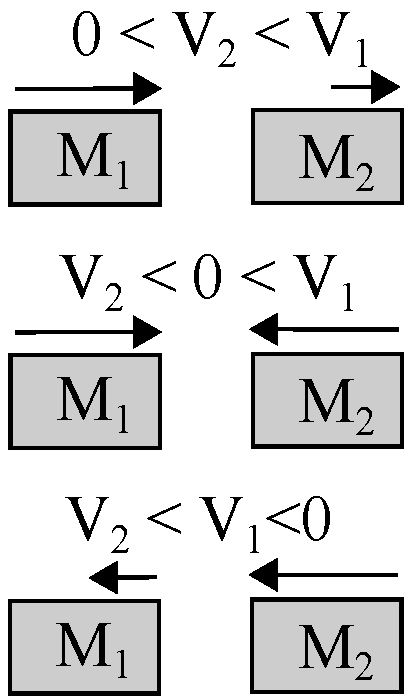
\includegraphics[width=0.17\linewidth]{Figs/little-momentum0.pdf} 
 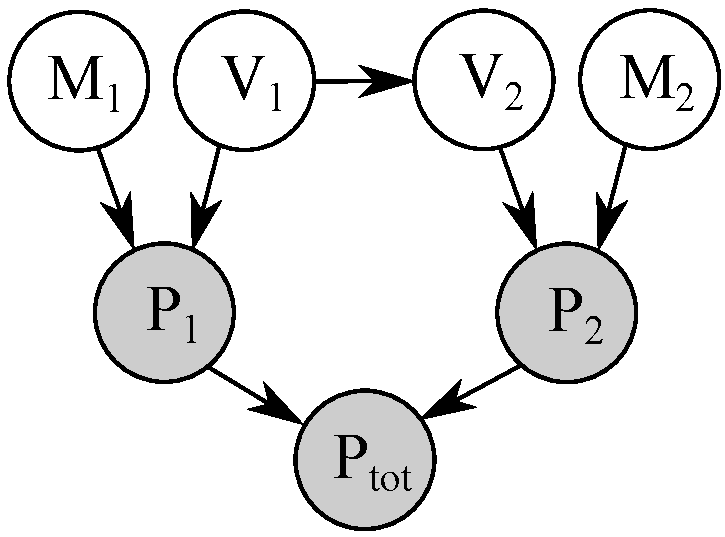
\includegraphics[width=0.33\linewidth]{Figs/little-momentum1.pdf} 
%\vspace{-0.05mm}
%\\
%\hspace{-5mm} \footnotesize(a) 
%& \hspace{-3mm} \footnotesize(b)  \\
%\multicolumn{2}{c}{}
%\end{tabular}
\end{center}
\vspace{-6mm}
\caption{\footnotesize
Bayesian network corresponding the \emph{collision model}. The filled circles represent deterministic random variables.} 
\label{fig:mom0}
\vspace{-2mm}
\end{figure}
%%%%%%%%%%%%%%%%%%%%%%%%%%%%%%%%%%%%%%%%%%%%%%%%%%%%%%%%%%%%%%%%%%%%%%%%%%


%%%%%%%%%%%%%%%%%%%
%%%%%%%%%%%%%%%%%%%
%\vspace{1mm}\\
{\bf Example (Collision model). }
\emph{Masses $M_1$ and $M_2$ with velocities $V_1$ and $V_2$ (and consequently momenta $P_1 = M_1 V_1$ and $P_2 = M_2 V_2$) collide to form a single mass ($M_1 + M_2$) with momentum $P_\text{tot} = P_1 + P_2$ (assuming that there is no dissipation).
Masses and velocities are unknown but 
their prior distributions are given as follows:\footnote{
Throughout, $\mathcal{U}(a, \, b)$ denotes a uniform continuous distribution 
with support interval $[a, b]$.
} 
%(note that as Figure~\ref{fig:mom0}.a shows, a collision only happens if $V_2 < V_1$):  
}%end \emph
{\footnotesize \vspace{-0.5mm}
\begin{align}
&\pr(M_1) = \mathcal{U}(0.1, \, 2.1) 
&&\pr(M_2) \!=\! \mathcal{U}(0.1, \, 2.1)
\nonumber
\\
&\pr(V_1) = \mathcal{U}(-2, \, 2)
&&\pr(V_2 \, | \, V_1) = \mathcal{U}(-2, \, V_1)
\label{e:collision}
\end{align} 
}
\emph{
\!\!\!The conditional dependencies of these random variables are illustrated in 
Figure~\ref{fig:mom0}. %b.
Conditioned on the observation $P_{\text{tot}} = 3$, the posterior joint distribution of $M_1$, $M_2$, $V_1$ and $V_2$ is desired. 
\hspace*{\fill} $\diamond$} %\emph

Despite its humble appearance, we will show the solutions that the existing probabilistic inference tools provide for this model are quite unsatisfactory. 

Let's take a closer look on the nature of the problem by manually carrying on the computations required for 
\emph{Markov chain Monte Carlo} (MCMC) sampling:
It can easily be seen that in the \emph{collision model}, 
the joint density of masses and velocities is
\begin{equation} \footnotesize  
\label{e:col-prior}
\pr(M_1, M_2, V_1, V_2)  
=
\begin{cases}
\frac{1}{16 V_1 + 32} &{\text{if }\scriptstyle 0.1<M_1<2.1, \, 0.1<M_2<2.1,}\\
							 &{\;\;\, \scriptstyle -2<V_1<2, \, -2<V_2 < V_1}\\
 \otherwise{0}
 \end{cases}
\end{equation}
which is a 4 dimensional function from which samples can be taken fairly easily. 
Since {\footnotesize $P_\text{tot} = M_1 V_1 + M_2 V_2$}, 
the following \emph{likelihood} is a 0-variance conditional distribution:
\begin{equation}\footnotesize 
\label{e:col-likelihood}
\pr(P_\text{tot} = 3 \,|\, M_1, V_1, M_2, V_2) = \delta( M_1 V_1 + M_2 V_2 - 3)
\end{equation}
where $\delta(\cdot)$ denotes \emph{Dirac delta}. 
By \emph{Bayes} rule, 
the \emph{posterior} 
{\footnotesize $\pr(M_1, M_2, V_1, V_2 \,|\, P_\text{tot} = 3)$}
is proportional to the product of equations (\ref{e:col-prior}) and (\ref{e:col-likelihood}).
Note that despite being 4-dimensional, 
the mass of this function is only non-zero on the 3 dimensional \emph{hypersurface}: {\footnotesize$M_1 V_1 + M_2 V_2 = 3$}. 


In general, observation of an algebraic relationship between random variables of an {\footnotesize$N$}-dimensional prior space often corresponds a zero-probability event that leads to a posterior mass positioned on an {\footnotesize$(N\!-\!1)$}-dimensional hyperspace and conditioning on multiple such events increases the difference between the dimensionality of the original space and the \emph{submanifold} on which the posterior is non-zero.  
If this dimensionality mismatch is not taken into account, sampling from such posterior distributions via sampling will be impossible (As a more tangible example, note that taking sample from a 2D curve via random walk in a 3D continuous space is impossible.)  

%We are unaware of any off-the-shelf inference framework that handles conditioning on deterministic constraints among random variables.
\subsection{Literature review}
By imposing various %(but functionally the same)
\emph{syntactical restrictions}, % and excuses, 
the state-of-the-art probabilistic programming languages (PPLs),
%totally 
disallow deterministic relationships among continuous random variables 
(a.k.a.\ deterministic constraints) be observed.\footnote{
In BUGS \citep{lunn2009bugs}, the popular software for analysis of statistical models, \emph{logical nodes} cannot be given data or initial values .
In PyMC \citep{patil2010pymc} deterministic variables have no \emph{observed flag}. 
In Stan \citep{stan-manual:2014} 
if you try to assign an observation value to a deterministic variable, you will encounter an error message: 
``attempt to assign variable in wrong block'' while 
Anglican \citep{wood2014new} throws error ``invalid-observe", etc.}

The solution that these off-the-shelf inference frameworks suggest is to approximate the observed determinism via adding noise to the observation 
(hard to soft constraint conversion via introducing measurement error).

For example the r.h.s of equation (\ref{e:col-likelihood}) would be 
approximated with a normal distribution
{\footnotesize $\mathcal{N}( M_1 V_1 + M_2 V_2 - 3, \sigma_\eta^2)$}  
where the variance $\sigma_\eta^2$ is the noise parameter.

Using this trick, it is guaranteed that the posterior is equidimensional with the (space of) prior (i.e.\ its ambient space) and therefore in theory, conventional (MC)MC sampling is possible.
Nonetheless, in practice such an strategy may not help much:
If the added noise is large, 
the approximation bounds may become arbitrarily large
and if the noise is small, 
the mixing rate may become extremely slow \citep{chin1987bayesian}. 
The reason is that in the latter case, 
 the approximated posterior mass would be dense in tinny regions (surrounding the original submanifold) on which random walk
is notoriously inefficient (near-deterministic problem).  

%If all stochastic distributions of the model belong to particular families of density functions, the problem may be addressed by means of  
%\emph{variable transformations}.
In particular settings, \emph{linear} deterministic relationships between continuous random variables
are addressed in the literature.  
Most notably, 
the family of \emph{conditional linear Gaussians (CLGs)} \citep{lauritzen2001stable}, 
i.e\ constant-variance \emph{Gaussian} densities where the mean of each random variable is a linear function of its parents,
is closed under linear transformations and consequently
allow linear deterministic constraints.%\footnote{CLGs form constant-variance \emph{Gaussian} Bayesian networks where the mean of each stochastic random variable is a linear function of its parents. \citep{lauritzen2001stable}.}

In \citep{li2013dynamic} the restriction is imposed on the network topology.
They use \emph{sequential importance sampling} on a simple Bayesian network of i.i.d. data points with an observed summation. % in a minimalistic BN.
%They conjecture that such an algorithm may be generalized to other settings. 
The generalization of this technique does not seem straight-forward (if possible).
%It is unknown if this technique can be generalized to other topologies and evidence. 

Recently, piecewise polynomial distributions have attracted attention.
So far, piecewise polynomials with hyperrectangular, hyper-rhombus and linear partitioning constraints have been used in Bayesian networks \citep{shenoy2011inference,shenoy2012two,Sanner:12}.
Such families can handle linear deterministic conditionals.
\cite{cobb2005nonlinear} approximate non-linear deterministic constraints with piecewise linear constraints via
dividing the domain of the parent variables into hypercubes. % and creating an approximation of each function in each hypercube.
This method is not scalable and rapidly loses its performance in high dimensions since 
the number of partitions required to preserve approximation accuracy
grows exponentially in the variable space dimensionality. 

In short, inference conditioned on nonlinear deterministic relationships between continuous random variables is still an open problem \citep{li2013dynamic} and as mentioned, even for linear constraints, the existing works are too restrictive.
 
\subsection{Contribution and outline}
In this paper, we provide an efficient automatic inference mechanism 
on an expressive class of continuous distributions 
that handles a large class of linear and nonlinear multivariate algebraic deterministic relationships between continuous random variables that are in the form of polynomial fractions. 

After a brief background to %representation and inference in 
graphical models (GMs) in Section~\ref{sect:background}, 
%our first main contributions is presented in Section~\ref{sect:contribution1} where 
in Section~\ref{sect:contribution1} we provide the necessary theory and algorithm (called \emph{collapsing determinism}) 
to transform models with a large class of (observed) deterministic constraints to purely stochastic networks. % for a large set of (non)linear algebraic determinism. 
%The main idea is to reduce the posterior dimensionality by utilizing the properties of Dirac delta distributions. This algorithm relies on operations such as fractional substitutions. It can easily be seen that under such operations, the typical classes of distributions that are studied in the literature so far do not remain closed. This should be the main reason why the problem of inference conditioned on determinism has remained {\color{green}untackled} so far. 
It can be seen that the classes of distributions studied in the literature so far do not remain closed under operations (such as fractional substitutions) required for collapsing determinism.
This is remedied in 
%Our second contribution is presented in 
Section~\ref{sect:ppfs} where we 
%{\color{green}alleviate} this situation as follows:\bf We 
introduce \emph{polynomial piecewise fractions} (PPFs), a highly expressive class of functions, not studied in the literature so far, 
with interesting properties that facilitate the inference conditioned on deterministic algebraic constraints.

%This class (called PPFs for \emph{polynomial piecewise fractions}) {\color{green}consists of} piecewise functions where the space of variables is partitioned by polynomial inequalities and the the function value in each partition is a fraction with a polynomial numerator and denominator.  
%Clearly, PPFs can approximate any function up to arbitrary precision by partitioning it into (relatively) {\color{green} homogeneous} pieces followed by utilizing \emph{Taylor} expansion or similar methods.
%The key insight is that PPFs are closed under derivation and polynomial fractional substitutions. This immediately extends their application to models with sophisticated algebraic constraints.

%Unfortunately, PPFs are not closed under integration (required for marginalization). Therefore, closed-form inference on PPF models is not in general possible.  Nonetheless, 

A large subset of PPFs have closed-form univariate symbolic integrals which leads to another contribution
presented in Section~\ref{sect:symbolic.gibbs}: %our third contribution: In Section~\ref{sect:symbolic.gibbs}, we propose 
performing 
the costly operation of univariate CDF computation, as required by Gibbs sampling, analytically and offline rather than per sample.     
%Gibbs samplers are robust in the sense that they do not need any parameter tuning.However, they are computationally expensive since to take a single sample they require to compute many univariate integrals (to generate the CDFs of conditional distributions).
%We notice that a large subset of PPFs have closed form (symbolic) integrals. 
%The idea of Symbolic Gibbs is to compute a single analytic integral for each variable by keeping the remaining variables uninstantiated. 
%The actual process of CDF computation per sample  simply involves instantiation of the already computed CDFs rather than computing them on the fly.
This dramatically decreases the amount of necessary computations and as our experimental results in Section~\ref{sect:experimental.results} show, 
leads to a significant improvement in the convergence rates. 
%Literature review is postponed to Section~\ref{sect:literature.review} and 
The summary and conclusion are offered in Section~\ref{sect:conclusion}. 

%In the following sections after a brief introduction to Graphical models, followed by an algorithm for inference in the presence of deterministic constraints.We then explain the restrictions of PPFs, compare our method with other samplers and conclude. 
